% !TEX encoding = UTF-8 Unicode
% !TEX TS-program = pdflatex
% !TEX root = ../Tesi.tex



%************************************************
\myChapter{Specchio e sistema di controllo}
%************************************************
\label{chap:mirror}
Al fine di poter valutare il comportamento del gruppo di controllo analizzato nel Capitolo \ref{chap:ActSens} è stato sviluppato un codice di simulazione strutturale di uno specchio attivo. La scelta è ricaduta su un modello ampiamente utilizzato per prove sperimentali, chiamato \textit{P45} \citep{manettiphd}, integrato con il sistema di controllo digitale soggetto a disturbi opportunamente modellati. L'effetto dell'inserimento del comportamento degli attuatori e dei sensori verrà poi valutato sulle caratteristiche della risposta ad un caratteristico segnale temporale nel Capitolo \ref{chap:simulations}.

\section{Piastra di Mindlin}
Il codice strutturale ad elementi finiti è basato sul modello di piastra di Mindlin. Anche in questo caso sono state sfruttate le librerie di FEniCS per l'assemblaggio delle matrici di rigidezza.
Ai fini della caratterizzazione dello specchio è stato trascurato il movimento \textit{in plane} dello specchio, per il quale la stabilità non è garantita dal sistema di controllo bensì dal sostegno centrale. Nell'ipotesi di un disaccoppiamento completo fra il movimento trasversale e longitudinale, i gradi di libertà considerati identificano tre campi scalari:
\begin{equation}
\label{eq:7plv1}
\T{u} = \left\{
\begin{array}{c}
w\\ \theta_x\\ \theta_y\end{array}\right\},
\end{equation}
dove $w$ è lo spostamento perpendicolare al piano, $\theta_x$ e $\theta_y$ sono, rispettivamente, le rotazioni della sezione attorno agli assi $x$ e $y$ del sistema di riferimento. 

Il lavoro virtuale delle forze elastiche per i gradi di libertà considerati, assumendo stato piano di sforzo e materiale isotropo, può essere scritto come segue:
\begin{align}
\label{eq:7plv2}
&\delta \TTTT{L}_d =\nonumber\\&=
\int_V\delta\left\{
\begin{array}{c}
z \de_x\theta_y\\ 
-z \de_y\theta_x\\ 
z \left(\de_x\theta_x- \de_y\theta_y\right)\\
\theta_y+\de_x w\\
-\theta_x+\de_y w
\end{array}\right\}\cdot
\left\{
\begin{array}{c}
\frac{Ez}{1-\nu^2}\left(\de_x\theta_y- \nu\de_y\theta_x\right)\\
\frac{Ez}{1-\nu^2}\left(\nu\de_x\theta_y- \de_y\theta_x\right)\\
-z G \left(\de_x\theta_x- \de_y\theta_y\right)\\
G\left(\theta_y+\de_x w\right)\\
G\left(-\theta_x+\de_y w\right)
\end{array}\right\}dv,
\end{align}
dove:
\begin{equation}
\label{eq:7plv3}
\left\{\begin{array}{l}
E\text{ è il modulo di Young}\\
\nu\text{ è il coefficiente di Poisson}\\
G = \frac{E}{2\left(1+\nu\right)}\text{ è il modulo di rigidezza a taglio.}
\end{array}\right.\nonumber
\end{equation}

Riorganizzando l'equazione e isolando i contributi flessionali e di taglio si ottiene:
\begin{equation}
\label{eq:7plv4}
\delta \TTTT{L}_d = \int_V\left(\delta\T{\varepsilon_{fl}}\cdot\TT{\hat{E}_{fl}}\T{\varepsilon_{fl}} +G\delta\T{\varepsilon_{t}}\cdot\T{\varepsilon_{t}}\right)dv,
\end{equation}
con
\begin{align}
\label{eq:7plv5}
&\T{\varepsilon_{fl}} = \left\{
\begin{array}{c}
\de_x\theta_y\\ 
\de_y\theta_x\\ 
\de_x\theta_x- \de_y\theta_y
\end{array}\right\},\\
\label{eq:7plv5bis}
&\TT{\hat{E}_{fl}} = \frac{Ez^2}{1-\nu^2}\left[\begin{array}{ccc}
1 & -\nu & 0\\-\nu & 1 & 0\\0&0& \frac{G\left(1-\nu^2\right)}{E}\end{array}\right],\\
\label{eq:7plv5tris}
&\T{\varepsilon_{t}} = \left\{
\begin{array}{c}
\theta_y+\de_x w\\ 
-\theta_x+\de_y w
\end{array}\right\}.
\end{align}

Dividendo l'integrale di volume, si ha:
\begin{align}
\label{eq:7plv6}
\delta \TTTT{L}_d &= \int_A\int_{-t/2}^{t/2}\left(\delta\T{\varepsilon_{fl}}\cdot\TT{\hat{E}_{fl}}\T{\varepsilon_{fl}} +G\delta\T{\varepsilon_{t}}\cdot\T{\varepsilon_{t}}\right)dzdA\\
\label{eq:7plv6bis} &= \int_A\left(\delta\T{\varepsilon_{fl}}\cdot\TT{E_{fl}}\T{\varepsilon_{fl}} +Gt\delta\T{\varepsilon_{t}}\cdot\T{\varepsilon_{t}}\right)dA,
\end{align}
dove 
\begin{equation}
\label{eq:7plv7}
\TT{\hat{E}_{fl}} = \frac{Et^3}{12\left(1-\nu^2\right)}\left[\begin{array}{ccc}
1 & -\nu & 0\\-\nu & 1 & 0\\0&0& \frac{G\left(1-\nu^2\right)}{E}\end{array}\right].
\end{equation}

Il lavoro delle forze d'inerzia può essere espresso come\footnote{Per semplificare la notazione, in ambito strutturale si preferisce indicare la derivata temporale di una quantità $x$ con $\dot{x}$ anziché $\de_t x$.}:
\begin{align}
\label{eq:7plv8}
\delta\TTTT{L}_i &=-\int_A \int_{-t/2}^{t/2} \delta\T{u}
\cdot
\left[
\begin{array}{ccc}
\rho & \rho z & \rho z \\
\rho z & \rho z^2 & 0 \\
\rho z & 0 & \rho z^2
\end{array}
\right]\ddot{\T{u}}~dzdA\\
\label{eq:7plv8.1}
& = 
-\int_A \delta\T{u}
\cdot
\left[
\begin{array}{ccc}
\rho t & 0 & 0 \\
0 & \rho\frac{t^3}{12} & 0 \\
0 & 0 & \rho \frac{t^3}{12}
\end{array}
\right]\ddot{\T{u}}~dA\\
\label{eq:7plv8.2}
 &=- \int_A \delta\T{u} \TT{M_l}\ddot{\T{u}}~dA.
\end{align}
Il contributo di masse e inerzie concentrate può essere aggiunto:
\begin{align}
\label{eq:7plv8bis}
\delta\TTTT{L}_i &=-\delta\T{u}\left(x_P,y_P\right)
\cdot \TT{M_P}~\ddot{\T{u}}\left(x_P,y_P\right)\\
\label{eq:7plv8bis2}
&= \lfloor\T{u}\cdot \TT{M_P}~\ddot{\T{u}} \rfloor_{\left(x_P,y_P\right)}.
\end{align}
Infine, il lavoro delle forze e coppie esterne può essere scritto, separando contributi superficiali e concentrati, come:
\begin{align}
\label{eq:7plv9}
\delta\TTTT{L}_e &=\int_A \delta\T{u}
\cdot \left\{\begin{array}{c}f_z\\c_x\\c_y\end{array}\right\}dA 
+ \delta\T{u}\left(x_P,y_P\right)
\cdot \left\{\begin{array}{c}F_z\left(x_P,y_P\right)\\C_x\left(x_P,y_P\right)\\C_y\left(x_P,y_P\right)\end{array}\right\}\\
& = 
\int_A \delta\T{u}
\cdot
\T{f}~dA+\lfloor\T{u}\cdot \T{F} \rfloor_{\left(x_P,y_P\right)}.
\end{align}
La dinamica della piastra può essere allora espressa tramite l'equazione in forma variazionale:
\begin{equation}
\label{eq:7plv10}
\delta \TTTT{L}_d = \delta \TTTT{L}_i + \delta \TTTT{L}_e
\end{equation}


Per lo smorzamento strutturale viene utilizzato il modello proporzionale:
\begin{equation}
\label{eq:7plv11}
\TT{C} = \alpha \TT{M}+\beta\TT{K}.
\end{equation}

I valori $\alpha$ e $\beta$ sono stati ottenuti imponendo due valori di fattore di smorzamento desiderati $\xi_{1,2}$ per due pulsazioni caratteristiche $\omega_{1,2}$ e risolvendo il sistema lineare:
\begin{equation}
\label{eq:7plv12}
\left\{
\begin{array}{c}
2\xi_1\omega_1 = \alpha+\beta\omega_1^2\\
2\xi_2\omega_2 = \alpha+\beta\omega_2^2\\
\end{array}\right.
\end{equation}

I valori sono stati scelti per rappresentare i contributi di dissipazione strutturale e fluidodinamica.\\

Per non incorrere nel fenomeno dello \textit{shear locking} (e la conseguente erronea distribuzione dei contributi energetici di deformazione fra flessione e taglio) è sufficiente porre attenzione agli ordini degli elementi per gli spazi funzionali considerati: in particolare, gli elementi del campo $w$ devono essere superiori agli altri di almeno un ordine. In questo lavoro si è fatto uso di elementi lagrangiani di ordine 3 per lo spostamento $w$ e di ordine 2 per le rotazioni $\theta_x$ e $\theta_y$.

Assemblando le matrici, il sistema assume la consueta forma:

\begin{equation}
\label{eq:7plv13}
\TT{M}\ddot{\T{x}}+\TT{C}\ddot{\T{x}}+\TT{K}\T{x} = \T{q}.
\end{equation}
\subsection{Test-case: pannello rettangolare}

In questa sezione verrà validato il modello strutturale mediante confronti con il solutore commerciale MSC Nastran. I confronti riguardano analisi statiche con carichi distribuiti o concentrati ed estrazioni modali. 

Il confronto è stato effettuato per un pannello rettangolare. I dati geometrici e strutturali del pannello sono elencati in Tabella \ref{tab:7rettangolo1}.\\

\begin{table}[htb]
\caption{Pannello rettangolare: dati del modello}
\label{tab:7rettangolo1}
\centering
\begin{tabular}{lcc}
\toprule
Lato 1 & $l_x$ & 10 m \\
Lato 2 & $l_y$ & 5 m \\
Modulo di Young & $E$ & 72 GPa\\
Coeff. di Poisson & $\nu$ & 0.3\\
Forza verticale nel nodo $A$& $F_A$ & 3 N\\
Forza verticale nel nodo $B$& $F_B$ & -2 N\\
\bottomrule
\end{tabular}
\end{table}

Come prima analisi, è stato imposto un vincolo d'incastro su uno dei lati corti e applicati due carichi concentrati di entità diversa agli estremi del lato opposto a quello vincolato. Questa condizione è utile per la verifica dell'assenza di \textit{shear-locking}.

Lo spostamento ottenuto con i due codici è riportato in Tabella \ref{tab:7rettangolo2}. Come si può vedere, le differenze sono estremamente basse; la soluzione è sostanzialmente coincidente.

\begin{figure}[h]
\centering
\caption{Pannello rettangolare soggetto a carichi concentrati: confronto sulla deformata }
\label{fig:7rettangolowconf}
\subfloat[][FEniCS]{

\includegraphics[width = .48\textwidth]{rettangolow}}
\subfloat[][Nastran]{

\includegraphics[width = .38\textwidth]{rettangolownastran}}
\end{figure}


\begin{table}[h]
\caption{Pannello rettangolare soggetto a carichi concentrati: confronto fra gli spostamenti massimi}
\label{tab:7rettangolo2}
\centering
\begin{tabular}{lc}
\toprule
~&Spostamento del nodo $A$\\
FEniCS & 2.0799 m\\
Nastran & 2.0787 m\\
\bottomrule
\end{tabular}
\end{table}


In seguito, per verificare la corretta integrazione delle forze superficiali, sul pannello sono stati applicati un vincolo di appoggio su tutti i lati e una pressione costante pari a 0.05 Pa. 

Lo scostamento massimo è mostrato in Tabella \ref{tab:7rettangolo3}. Anche in questo caso le soluzioni sono sostanzialmente coincidenti.

\begin{figure}[h]
\centering
\caption{Pannello rettangolare soggetto a carichi distribuiti: confronto sulla deformata}
\label{fig:7rettangolowconf2}
\subfloat[][FEniCS]{

\includegraphics[width = .48\textwidth ]{rettangolowpressure}}
\subfloat[][Nastran]{

\includegraphics[width = .38\textwidth]{rettangolowpressurenastran}}
\end{figure}


\begin{table}[htb]
\caption{Pannello rettangolare soggetto a carichi distribuiti: confronto fra gli scostamenti massimi}
\label{tab:7rettangolo3}
\centering
\begin{tabular}{lc}
\toprule
~&Scostamento del nodo centrale (massimo)\\
FEniCS & 5.88 mm\\
Nastran & 5.89 mm\\
\bottomrule
\end{tabular}
\end{table}


Infine, in Tabella \ref{tab:7rettangolo4}, si riportano le frequenze ottenute per i primi 20 autovalori in una analisi modale del pannello libero (non smorzato). 

\begin{table}[h]
\caption{Pannello rettangolare: confronto fra le frequenze dei primi 20 modi di vibrare}
\label{tab:7rettangolo4}
\centering
\begin{tabular}{lcclcc}
\toprule
& FEniCS & Nastran &  & FEniCS & Nastran\\
\midrule
1° &  0.00000    Hz & 0.00000   Hz   &   11° &  0.59397     Hz &  0.59384   Hz \\
2° &  0.00000    Hz & 0.00000   Hz   &   12° &  0.71837     Hz &  0.71796   Hz \\
3° &  0.00000    Hz & 0.00000   Hz   &   13° &  0.79599     Hz &  0.79559   Hz \\
4° &  0.10688    Hz & 0.10687   Hz   &   14° &  0.96473     Hz &  0.96420   Hz \\
5° &  0.13084    Hz & 0.13080   Hz   &   15° &  1.01235     Hz &  1.01192   Hz \\
6° &  0.28880    Hz & 0.28870   Hz   &   16° &  1.16824     Hz &  1.16753   Hz \\
7° &  0.29720    Hz & 0.29715   Hz   &   17° &  1.22971     Hz &  1.22906   Hz \\
8° &  0.44063    Hz & 0.44049   Hz   &   18° &  1.30786     Hz &  1.30711   Hz \\
9° &  0.50297    Hz & 0.50276   Hz   &   19° &  1.32918     Hz &  1.32802   Hz \\
10° & 0.51933    Hz & 0.51911   Hz   &   20° &  1.47560     Hz &  1.47435   Hz \\
\bottomrule
\end{tabular}
\end{table}
\clearpage
\section{Schema di controllo}
I sistemi di controllo per gli specchi attualmente in uso devono far fronte a diverse problematiche fra cui l'alta densità modale e il basso smorzamento dei modi ad alta frequenza. Inoltre l'acquisizione, l'elaborazione dei segnali e l'applicazione degli ingressi di controllo richiedono un tempo troppo lungo per un'architettura a ciclo chiuso centralizzata. Per questo la struttura è a più livelli: il segnale di posizione di riferimento elaborato sulla base della misura della distorsione del fronte d'onda viene inviato a tutti gli attuatori mediante un controllo in \textit{feed-forward} centralizzato a frequenza definita sulla base dei tempi caratteristici delle distorsioni (per specchi terrestri, dove la fonte di disturbo più rapida è la turbolenza atmosferica, la frequenza di aggiornamento è variabile tra 1 e 2 kHz). Un ciclo di retroazione decentralizzato a frequenza più alta (attualmente nell'ordine del centinaio di kHz) assicura l'inseguimento del segnale con scostamenti
massimi di 10--20 nm.


Questa architettura permette di sfruttare i vantaggi del controllo
decentralizzato in ciclo chiuso, in particolare l'elevata velocità di elaborazione e la
robustezza rispetto a disturbi ed errori di modellazione, per stabilizzare la forma dello specchio nell'intorno della posizione desiderata \citep{manetti_high_2010}.

\begin{figure}[htb]
\centering
\caption{Raccordo per il segnale in \textit{feed-forward}}
\label{fig:71menocos}
\begin{tikzpicture}
\begin{axis}[width = .8\textwidth,
             height = .2\textheight,             
             ylabel = $f_{sh}$,
			 xlabel = $t$,
			 ticks = none, 
			 ymax = 1.2,
			 axis x line = middle, 
			 axis y line = middle, 
			 enlargelimits,
			 semithick]
\addplot[thick, smooth, samples = 200,domain = 0:180]
{0.5*(1-cos(x))};
\addplot[thick, smooth, samples = 100,domain = 180:500]
{1};
\end{axis}
\end{tikzpicture}
\begin{tikzpicture}
\begin{axis}[width = .8\textwidth,
             height = .2\textheight,  
             ylabel = $\dot{f}_{sh}$,
			 xlabel = $t$,
			 ticks = none, 
			 ymax = 1.2,
			 axis x line = middle, 
			 axis y line = middle, 
			 enlargelimits,
			 semithick]
\addplot[thick, smooth, samples = 200,domain = 0:180]
{sin(x)};
\addplot[thick, smooth, samples = 200,domain = 180:500]
{0};
\end{axis}
\end{tikzpicture}
\begin{tikzpicture}
\begin{axis}[width = .8\textwidth,
             height = .2\textheight,  
             ylabel = $\dot{f}_{sh}$,
			 xlabel = $t$,
			 ticks = none, 
			 ymax = 1.2,
			 axis x line = middle, 
			 axis y line = middle, 
			 enlargelimits,
			 semithick]
\addplot[thick, smooth, samples = 200,domain = 0:180]
{cos(x)};
\addplot[thick, smooth, samples = 200,domain = 180:500]
{0};
\draw {(180,-1)--(180,0)};
\end{axis}
\end{tikzpicture}
\end{figure}

Il segnale di riferimento elaborato è inviato con frequenza $f_{ol}$ e viene mantenuto costante per la durata di un ciclo ($T_{ol} = 1/f_{ol}$). Il segnale complessivo di riferimento per ogni attuatore risulta composto da tratti costanti, che vengono opportunamente raccordati utilizzando funzioni polinomiali o trigonometriche (Figura \ref{fig:71menocos}). Definendo $\T{d_k^r}$ il vettore contenente le posizioni di riferimento al passo corrente per i punti di controllo e $\T{d_{k+1}^r}$ il vettore delle posizioni al passo successivo, la storia temporale da inseguire è:


\begin{align}
\label{eq:7ff1}
\T{r}(t) &= \T{d_k^r}+\left(\T{d_{k+1}^r} -\T{d_k^r}\right)f_{sh}(t)\\
\label{eq:7ff1.0}
\dot{\T{r}}(t) &= \left(\T{d_{k+1}^r} -\T{d_k^r}\right)\dot{f}_{sh}(t)\\
\label{eq:7ff1.1}
\ddot{\T{r}}(t) &= \left(\T{d_{k+1}^r} -\T{d_k^r}\right)\ddot{f}_{sh}(t),
\end{align}
dove $f_sh$ è la funzione di raccordo (\textit{shaping}) normalizzata, tale per cui:
\begin{equation}
\label{eq:7ff2}
\left\{\begin{array}{c}
f_{sh}(0) = 0\\
f_{sh}(\hat{T}) = 1\\
\dot{f}_{sh}(0) = 0\\
\dot{f}_{sh}(\hat{T}) = 0
\end{array}\right.
\end{equation}
e $\hat{T}$ è un tempo caratteristico per il raccordo; per le simulazioni successive è stato utilizzato:
\begin{equation}
\label{eq:7ff3}
\hat{T} = \frac{T_{ol}}{4}.
\end{equation}

Il vettore delle forze in anello aperto è elaborato approssimando la dinamica strutturale sulla base di matrici di rigidezza, massa e smorzamento identificate sperimentalmente $\TT{K^*}$, $\TT{M^*}$, $\TT{C^*}$. Tali matrici sono  simili alle matrici condensate rispetto ai punti di controllo, e differiscono soltanto per l'effetto non lineare della non co-locazione di sensori e attuatori.
\begin{align}
\label{eq:7ff4}
\T{F_{ol}}(t) =& \TT{M^*}\ddot{\T{r}}(t)+\TT{C^*}\dot{\T{r}}(t)+\TT{K^*}\T{r}(t)\nonumber\\
=& \TT{M^*}\left(\T{d_{k+1}^r} -\T{d_k^r}\right)\ddot{f}_{sh}(t)+\nonumber\\
&+\TT{C^*}\left(\T{d_{k+1}^r} -\T{d_k^r}\right)\dot{f}_{sh}(t)+\nonumber\\
&+\TT{K^*}\left[\T{d_k^r}+\left(\T{d_{k+1}^r} -\T{d_k^r}\right)f_{sh}(t)\right].
\end{align}

 
Al contributo del controllore in ciclo aperto viene aggiunto il controllo decentralizzato basato su architettura PD. Identificando con $\tilde{\T{w}}$ il vettore degli spostamenti trasversali $w$ misurati dai sensori, le forze in anello chiuso possono essere scritte come:
\begin{align}
\label{eq:7fb1}
\T{F_{cl}}(t) = \TT{G_p}\left[\T{r}(t)-\tilde{\T{w}}(t)\right]+ \TT{G_d}\left[\dot{\T{r}}(t)-\dot{\tilde{\T{w}}}(t)\right].
\end{align}

Le matrici dei guadagni hanno struttura completamente diagonale per l'architettura de-centralizzata. L'implementazione digitale a tempo discreto del controllo impone l'utilizzo delle misure acquisite nel passo di campionamento precedente. Questo comporta l'introduzione di un ritardo costante nell'applicazione del controllo proporzionale. Il vettore $\dot{\tilde{\T{w}}}$ è ricostruito numericamente con schemi alle differenze finite applicate ai valori di posizione acquisiti nei passi precedenti.

Negli specchi attuali è comune l'introduzione di un contributo integrale, che può essere ottenuto sia attraverso il controllo in ciclo chiuso (aggiungendo il contributo allo schema \textit{PD}), sia attraverso l'utilizzo di un contributo ricorsivo in anello aperto detto controllo \textit{ossimorinico} o \textit{ibrido} \citep{manetti_self-tuning_2014}. In questo lavoro è stato implementato il secondo metodo: considerando il passo di controllo $k$, nella fase in cui la posizione viene mantenuta statica viene registrata una media della misura dello spostamento del punto di controllo. Questa media viene utilizzata per la costruzione del contributo di forza in feed-forward al passo $k+1$: la forza inviata dal controllore centralizzato non è più propriamente in anello aperto poiché contiene delle informazioni sullo stato del sistema. Il contributo ibrido si ottiene sostituendo il valore mediato $\T{\bar{w}}_k$ a $d^r_k$ e sostituendo il termine statico $\TT{K^*}\bar{\T{w}}_k$ con la forza media $\bar{\T{F}}_k$ (le medie sono calcolate nella fase finale del passo precedente, in cui la posizione è mantenuta costante):

\begin{align}
\label{eq:7foxy}
\T{F_{oxy}}(t) =& \TT{M^*}\left(\T{d_{k+1}^r} -\T{\bar{w}}_k\right)\ddot{f}_{sh}(t)+\nonumber\\
&+\TT{C^*}\left(\T{d_{k+1}^r} -\T{\bar{w}}_k\right)\dot{f}_{sh}(t)+\nonumber\\
&+\TT{K^*}\left(\T{d_{k+1}^r} -\T{\bar{w}}_k\right)f_{sh}(t)+\bar{\T{F}}_k.
\end{align}


\section{Integratore implicito}

Per le simulazioni di risposta è stato implementato un metodo di integrazione implicito a due passi a dissipazione numerica modulabile \citep{masarati_efficient_2014}. Il metodo è così strutturato:
\begin{equation}
\label{eq:7metodo1}
x_{k+1} = a_0x_k+a_{-1}x_{k-1}+b_1\dot{x}_{k+1}+b_0\dot{x}_k+b_{-1}\dot{x}_{k-1},
\end{equation}
dove
\begin{align}
\label{eq:7metodo2.0}
&\alpha = \Delta t_p /\Delta t_c,\\
\label{eq:7metodo2.1}
&\beta = \alpha\frac{(2+\alpha)(1-\rho_\infty)^2+2(1+\alpha)(2\rho_\infty-1)}{2(1+\alpha)-(1-\rho_\infty)^2},\\
\label{eq:7metodo2.2}
&\delta = \frac{\alpha^2(1-\rho_\infty)^2}{2(2(1+\alpha)-(1-\rho_\infty)^2)},\\
\label{eq:7metodo2.3}
&a_0 = 1-\beta,\\
\label{eq:7metodo2.4}
&a_{-1} = \beta,\\
\label{eq:7metodo2.5}
&b_1 = \Delta t_c \left(\frac{\delta}{\alpha}+\frac{\alpha}{2}\right),\\
\label{eq:7metodo2.6}
&b_0 = \Delta t_c\left(\frac{\beta}{2}+\frac{\alpha}{2} -(1+\alpha)\frac{\delta}{\alpha}\right),\\
\label{eq:7metodo2.7}
&b_{-1} = \Delta t_c \left(\frac{\beta}{2}+\delta\right).\\
\end{align}

I parametri per la definizione delle costanti del metodo sono $\Delta t_p$ e $\Delta t_p$ (intervalli di avanzamento precedente e corrente) e $\rho_\infty$ (per la regolazione del filtraggio ad alte frequenze). Scegliendo opportunamente $\rho_\infty$ si bilanciano le proprietà di precisione alle basse frequenze e di filtraggio alle alte frequenze. Per la valutazione degli effetti di \textit{spill-over} si è scelto di limitare il filtraggio, utilizzando alle alte frequenze la sola dissipazione strutturale. Per questo sono stati usati valori di $\rho_\infty$ prossimi a 1. Applicando il metodo di integrazione al sistema strutturale \eqref{eq:7plv13} si ottiene:
\begin{equation}
\label{eq:7metodo3}
\left(\TT{M}+b_1\TT{C}+b_1^2\TT{K}\right)\ddot{\T{x}}_{k+1} = \T{q}_{k+1}-\TT{C}\T{v}_{k,k-1}-\TT{K}\T{u}_{k,k-1}\:,
\end{equation}
dove
\begin{align}
\label{eq:7metodo4.0}
\T{u}_{k,k-1} =& a_0\T{x}_k+a_{-1}\T{x}_{k-1}+\left(b_1a_0+b_0\right)\dot{\T{x}}_k+\nonumber\\
&+\left(b_1a_{-1}+b_{-1}\right)\dot{\T{x}}_{k-1}+ b_1b_0\ddot{\T{x}}_k+\nonumber\\
&+b_1b_{-1}\ddot{\T{x}}_{k-1},\\
\label{eq:7metodo4.1}
\T{v}_{k,k-1} =& a_0\dot{\T{x}}_k+a_{-1}\dot{\T{x}}_{k-1}+ b_0\ddot{\T{x}}_k+b_{-1}\ddot{\T{x}}_{k-1}.
\end{align}

\section{P45}

Come anticipato nell'introduzione di questo capitolo, la simulaizione del sistema di controllo è stata effettuata utilizzando i dati dello specchio $P45$, i cui dati geometrici e strutturali sono riportati in Tabella \ref{tab:7p45data}. Lo specchio è realizzato in \textit{Zerodur\sffamily\textregistered}, un materiale vetro-ceramico comune ad altre strutture adattive attualmente in uso. Il materiale è stato scelto per alcune proprietà importanti per le applicazioni ottiche, come il coefficiente di dilatazione termica quasi nullo e la possibilità di essere lucidato ad alti livelli di precisione.
Lo specchio possiede una debole curvatura che ai fini della simulazione del comportamento flessionale della piastra è trascurabile.\\

\begin{table}[hb]
\caption{Geometria e materiale per lo specchio $P45$}
\label{tab:7p45data}
\centering
\begin{tabular}{lc}
\toprule
Raggio interno & 0.12 m\\
Raggio esterno & 0.2834 m\\
Spessore & 1.61 mm\\
\midrule
Materiale & \textit{Zerodur\sffamily\textregistered}\\
\midrule
Modulo di Young & 91 GPa\\
Coefficiente di Poisson &  0.24\\
Densità & 2.53 g/$\text{cm}^3$\\
\bottomrule
\end{tabular}
\end{table}

La struttura è vincolata al centro attraverso una membrana elastica. Tuttavia questo vincolo è più rigido per i gradi di libertà \textit{in-plane} e il suo contributo trasversale può essere trascurato. Omettendo il vincolo centrale, la struttura è a tutti gli effetti labile e tenuta in equilibrio dinamico dalle sole forze di controllo.\\

\begin{figure}[htb]
\centering
\caption{Mappa dei punti di controllo per il $P45$: sensori (in grigio) e attuatori (in nero)}
\label{fig:7p45map}
\resizebox{.6\textwidth}{!}{
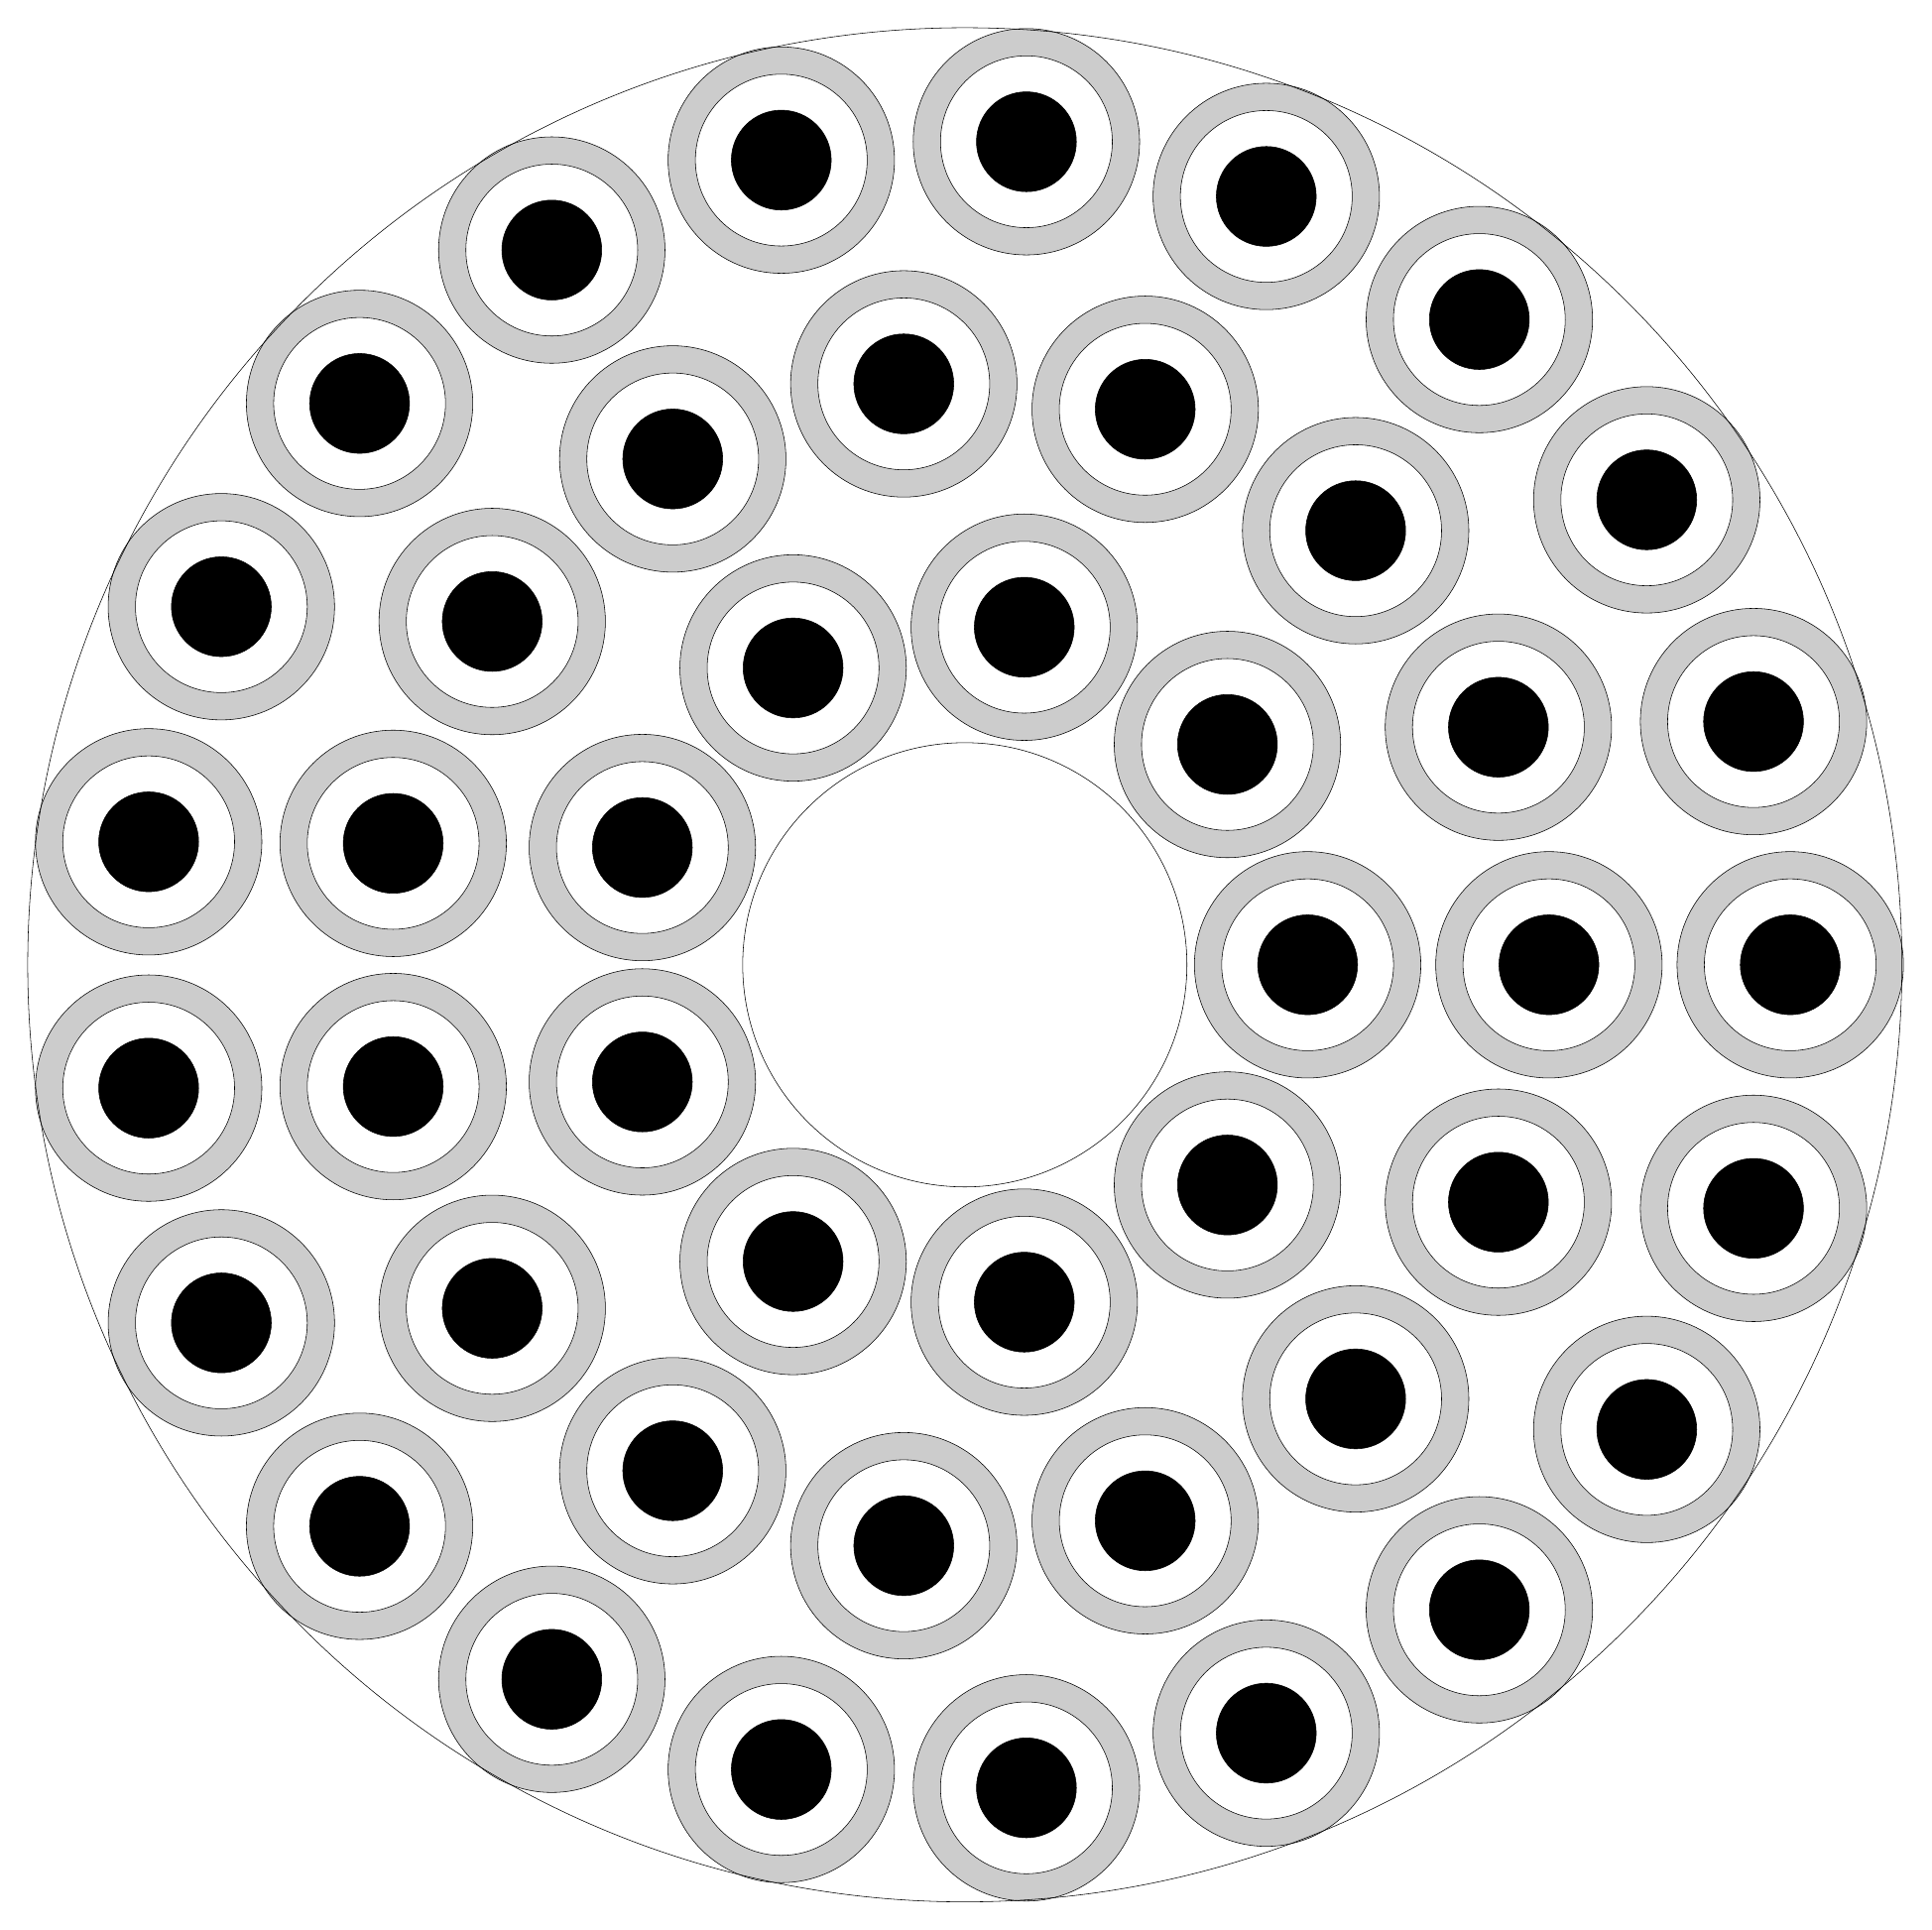
\begin{tikzpicture}
\filldraw[fill = black!20!white, draw = black, very thin](-2.35000e-02*100 , 1.03050e-01*100) circle(0.0145*100);
\filldraw[fill = black!20!white, draw = black, very thin](-5.29000e-02*100 , 9.15350e-02*100) circle(0.0145*100);
\filldraw[fill = black!20!white, draw = black, very thin](-9.52000e-02*100 , 4.58599e-02*100) circle(0.0145*100);
\filldraw[fill = black!20!white, draw = black, very thin](-1.04520e-01*100 , 1.57519e-02*100) circle(0.0145*100);
\filldraw[fill = black!20!white, draw = black, very thin](-1.04520e-01*100 ,-1.58000e-02*100) circle(0.0145*100);
\filldraw[fill = black!20!white, draw = black, very thin](-5.29000e-02*100 ,-9.14999e-02*100) circle(0.0145*100);
\filldraw[fill = black!20!white, draw = black, very thin]( 7.89899e-03*100 ,-1.05399e-01*100) circle(0.0145*100);
\filldraw[fill = black!20!white, draw = black, very thin]( 3.86149e-02*100 ,-9.83900e-02*100) circle(0.0145*100);
\filldraw[fill = black!20!white, draw = black, very thin](-7.74999e-02*100 , 7.18919e-02*100) circle(0.0145*100);
\filldraw[fill = black!20!white, draw = black, very thin]( 7.89899e-03*100 , 1.05399e-01*100) circle(0.0145*100);
\filldraw[fill = black!20!white, draw = black, very thin]( 6.59000e-02*100 , 8.26360e-02*100) circle(0.0145*100);
\filldraw[fill = black!20!white, draw = black, very thin]( 8.73300e-02*100 , 5.95409e-02*100) circle(0.0145*100);
\filldraw[fill = black!20!white, draw = black, very thin]( 1.01000e-01*100 , 3.11540e-02*100) circle(0.0145*100);
\filldraw[fill = black!20!white, draw = black, very thin]( 1.01000e-01*100 ,-3.11999e-02*100) circle(0.0145*100);
\filldraw[fill = black!20!white, draw = black, very thin]( 6.59000e-02*100 ,-8.26000e-02*100) circle(0.0145*100);
\filldraw[fill = black!20!white, draw = black, very thin](-7.74999e-02*100 ,-7.19000e-02*100) circle(0.0145*100);
\filldraw[fill = black!20!white, draw = black, very thin]( 6.83399e-02*100 ,-3.04000e-02*100) circle(0.0145*100);
\filldraw[fill = black!20!white, draw = black, very thin](-7.32000e-02*100 , 1.55530e-02*100) circle(0.0145*100);
\filldraw[fill = black!20!white, draw = black, very thin](-4.13000e-02*100 , 1.50160e-02*100) circle(0.0145*100);
\filldraw[fill = black!20!white, draw = black, very thin](-4.13000e-02*100 ,-1.49999e-02*100) circle(0.0145*100);
\filldraw[fill = black!20!white, draw = black, very thin](-6.05199e-02*100 , 4.39710e-02*100) circle(0.0145*100);
\filldraw[fill = black!20!white, draw = black, very thin]( 6.83399e-02*100 , 3.04269e-02*100) circle(0.0145*100);
\filldraw[fill = black!20!white, draw = black, very thin](-7.82000e-03*100 , 7.43970e-02*100) circle(0.0145*100);
\filldraw[fill = black!20!white, draw = black, very thin]( 2.31169e-02*100 , 7.11460e-02*100) circle(0.0145*100);
\filldraw[fill = black!20!white, draw = black, very thin]( 5.00560e-02*100 , 5.55929e-02*100) circle(0.0145*100);
\filldraw[fill = black!20!white, draw = black, very thin](-7.32000e-02*100 ,-1.55999e-02*100) circle(0.0145*100);
\filldraw[fill = black!20!white, draw = black, very thin](-7.82000e-03*100 ,-7.43999e-02*100) circle(0.0145*100);
\filldraw[fill = black!20!white, draw = black, very thin](-3.74000e-02*100 ,-6.47999e-02*100) circle(0.0145*100);
\filldraw[fill = black!20!white, draw = black, very thin]( 4.39039e-02*100 , 0.00000e+00*100) circle(0.0145*100);
\filldraw[fill = black!20!white, draw = black, very thin](-2.19999e-02*100 , 3.80220e-02*100) circle(0.0145*100);
\filldraw[fill = black!20!white, draw = black, very thin]( 7.62399e-03*100 ,-4.32000e-02*100) circle(0.0145*100);
\filldraw[fill = black!20!white, draw = black, very thin]( 7.62399e-03*100 , 4.32369e-02*100) circle(0.0145*100);
\filldraw[fill = black!20!white, draw = black, very thin]( 3.36320e-02*100 , 2.82210e-02*100) circle(0.0145*100);
\filldraw[fill = black!20!white, draw = black, very thin](-2.35000e-02*100 ,-1.03050e-01*100) circle(0.0145*100);
\filldraw[fill = black!20!white, draw = black, very thin]( 2.31169e-02*100 ,-7.11999e-02*100) circle(0.0145*100);
\filldraw[fill = black!20!white, draw = black, very thin](-9.52000e-02*100 ,-4.58599e-02*100) circle(0.0145*100);
\filldraw[fill = black!20!white, draw = black, very thin]( 1.05700e-01*100 , 0.00000e+00*100) circle(0.0145*100);
\filldraw[fill = black!20!white, draw = black, very thin]( 8.73300e-02*100 ,-5.94999e-02*100) circle(0.0145*100);
\filldraw[fill = black!20!white, draw = black, very thin](-6.05199e-02*100 ,-4.39999e-02*100) circle(0.0145*100);
\filldraw[fill = black!20!white, draw = black, very thin]( 5.00560e-02*100 ,-5.55999e-02*100) circle(0.0145*100);
\filldraw[fill = black!20!white, draw = black, very thin]( 7.48069e-02*100 , 0.00000e+00*100) circle(0.0145*100);
\filldraw[fill = black!20!white, draw = black, very thin](-3.74000e-02*100 , 6.47849e-02*100) circle(0.0145*100);
\filldraw[fill = black!20!white, draw = black, very thin]( 3.36320e-02*100 ,-2.81999e-02*100) circle(0.0145*100);
\filldraw[fill = black!20!white, draw = black, very thin](-2.19999e-02*100 ,-3.79999e-02*100) circle(0.0145*100);
\filldraw[fill = black!20!white, draw = black, very thin]( 3.86149e-02*100 , 9.83900e-02*100) circle(0.0145*100);
\filldraw[fill = white, draw = black, very thin](-2.35000e-02*100 , 1.03050e-01*100) circle(0.011*100);
\filldraw[fill = white, draw = black, very thin](-5.29000e-02*100 , 9.15350e-02*100) circle(0.011*100);
\filldraw[fill = white, draw = black, very thin](-9.52000e-02*100 , 4.58599e-02*100) circle(0.011*100);
\filldraw[fill = white, draw = black, very thin](-1.04520e-01*100 , 1.57519e-02*100) circle(0.011*100);
\filldraw[fill = white, draw = black, very thin](-1.04520e-01*100 ,-1.58000e-02*100) circle(0.011*100);
\filldraw[fill = white, draw = black, very thin](-5.29000e-02*100 ,-9.14999e-02*100) circle(0.011*100);
\filldraw[fill = white, draw = black, very thin]( 7.89899e-03*100 ,-1.05399e-01*100) circle(0.011*100);
\filldraw[fill = white, draw = black, very thin]( 3.86149e-02*100 ,-9.83900e-02*100) circle(0.011*100);
\filldraw[fill = white, draw = black, very thin](-7.74999e-02*100 , 7.18919e-02*100) circle(0.011*100);
\filldraw[fill = white, draw = black, very thin]( 7.89899e-03*100 , 1.05399e-01*100) circle(0.011*100);
\filldraw[fill = white, draw = black, very thin]( 6.59000e-02*100 , 8.26360e-02*100) circle(0.011*100);
\filldraw[fill = white, draw = black, very thin]( 8.73300e-02*100 , 5.95409e-02*100) circle(0.011*100);
\filldraw[fill = white, draw = black, very thin]( 1.01000e-01*100 , 3.11540e-02*100) circle(0.011*100);
\filldraw[fill = white, draw = black, very thin]( 1.01000e-01*100 ,-3.11999e-02*100) circle(0.011*100);
\filldraw[fill = white, draw = black, very thin]( 6.59000e-02*100 ,-8.26000e-02*100) circle(0.011*100);
\filldraw[fill = white, draw = black, very thin](-7.74999e-02*100 ,-7.19000e-02*100) circle(0.011*100);
\filldraw[fill = white, draw = black, very thin]( 6.83399e-02*100 ,-3.04000e-02*100) circle(0.011*100);
\filldraw[fill = white, draw = black, very thin](-7.32000e-02*100 , 1.55530e-02*100) circle(0.011*100);
\filldraw[fill = white, draw = black, very thin](-4.13000e-02*100 , 1.50160e-02*100) circle(0.011*100);
\filldraw[fill = white, draw = black, very thin](-4.13000e-02*100 ,-1.49999e-02*100) circle(0.011*100);
\filldraw[fill = white, draw = black, very thin](-6.05199e-02*100 , 4.39710e-02*100) circle(0.011*100);
\filldraw[fill = white, draw = black, very thin]( 6.83399e-02*100 , 3.04269e-02*100) circle(0.011*100);
\filldraw[fill = white, draw = black, very thin](-7.82000e-03*100 , 7.43970e-02*100) circle(0.011*100);
\filldraw[fill = white, draw = black, very thin]( 2.31169e-02*100 , 7.11460e-02*100) circle(0.011*100);
\filldraw[fill = white, draw = black, very thin]( 5.00560e-02*100 , 5.55929e-02*100) circle(0.011*100);
\filldraw[fill = white, draw = black, very thin](-7.32000e-02*100 ,-1.55999e-02*100) circle(0.011*100);
\filldraw[fill = white, draw = black, very thin](-7.82000e-03*100 ,-7.43999e-02*100) circle(0.011*100);
\filldraw[fill = white, draw = black, very thin](-3.74000e-02*100 ,-6.47999e-02*100) circle(0.011*100);
\filldraw[fill = white, draw = black, very thin]( 4.39039e-02*100 , 0.00000e+00*100) circle(0.011*100);
\filldraw[fill = white, draw = black, very thin](-2.19999e-02*100 , 3.80220e-02*100) circle(0.011*100);
\filldraw[fill = white, draw = black, very thin]( 7.62399e-03*100 ,-4.32000e-02*100) circle(0.011*100);
\filldraw[fill = white, draw = black, very thin]( 7.62399e-03*100 , 4.32369e-02*100) circle(0.011*100);
\filldraw[fill = white, draw = black, very thin]( 3.36320e-02*100 , 2.82210e-02*100) circle(0.011*100);
\filldraw[fill = white, draw = black, very thin](-2.35000e-02*100 ,-1.03050e-01*100) circle(0.011*100);
\filldraw[fill = white, draw = black, very thin]( 2.31169e-02*100 ,-7.11999e-02*100) circle(0.011*100);
\filldraw[fill = white, draw = black, very thin](-9.52000e-02*100 ,-4.58599e-02*100) circle(0.011*100);
\filldraw[fill = white, draw = black, very thin]( 1.05700e-01*100 , 0.00000e+00*100) circle(0.011*100);
\filldraw[fill = white, draw = black, very thin]( 8.73300e-02*100 ,-5.94999e-02*100) circle(0.011*100);
\filldraw[fill = white, draw = black, very thin](-6.05199e-02*100 ,-4.39999e-02*100) circle(0.011*100);
\filldraw[fill = white, draw = black, very thin]( 5.00560e-02*100 ,-5.55999e-02*100) circle(0.011*100);
\filldraw[fill = white, draw = black, very thin]( 7.48069e-02*100 , 0.00000e+00*100) circle(0.011*100);
\filldraw[fill = white, draw = black, very thin](-3.74000e-02*100 , 6.47849e-02*100) circle(0.011*100);
\filldraw[fill = white, draw = black, very thin]( 3.36320e-02*100 ,-2.81999e-02*100) circle(0.011*100);
\filldraw[fill = white, draw = black, very thin](-2.19999e-02*100 ,-3.79999e-02*100) circle(0.011*100);
\filldraw[fill = white, draw = black, very thin]( 3.86149e-02*100 , 9.83900e-02*100) circle(0.011*100);
                                                               
\filldraw[fill = black, draw = black, very thin](-2.35000e-02*100 , 1.03050e-01*100) circle(0.0064*100);
\filldraw[fill = black, draw = black, very thin](-5.29000e-02*100 , 9.15350e-02*100) circle(0.0064*100);
\filldraw[fill = black, draw = black, very thin](-9.52000e-02*100 , 4.58599e-02*100) circle(0.0064*100);
\filldraw[fill = black, draw = black, very thin](-1.04520e-01*100 , 1.57519e-02*100) circle(0.0064*100);
\filldraw[fill = black, draw = black, very thin](-1.04520e-01*100 ,-1.58000e-02*100) circle(0.0064*100);
\filldraw[fill = black, draw = black, very thin](-5.29000e-02*100 ,-9.14999e-02*100) circle(0.0064*100);
\filldraw[fill = black, draw = black, very thin]( 7.89899e-03*100 ,-1.05399e-01*100) circle(0.0064*100);
\filldraw[fill = black, draw = black, very thin]( 3.86149e-02*100 ,-9.83900e-02*100) circle(0.0064*100);
\filldraw[fill = black, draw = black, very thin](-7.74999e-02*100 , 7.18919e-02*100) circle(0.0064*100);
\filldraw[fill = black, draw = black, very thin]( 7.89899e-03*100 , 1.05399e-01*100) circle(0.0064*100);
\filldraw[fill = black, draw = black, very thin]( 6.59000e-02*100 , 8.26360e-02*100) circle(0.0064*100);
\filldraw[fill = black, draw = black, very thin]( 8.73300e-02*100 , 5.95409e-02*100) circle(0.0064*100);
\filldraw[fill = black, draw = black, very thin]( 1.01000e-01*100 , 3.11540e-02*100) circle(0.0064*100);
\filldraw[fill = black, draw = black, very thin]( 1.01000e-01*100 ,-3.11999e-02*100) circle(0.0064*100);
\filldraw[fill = black, draw = black, very thin]( 6.59000e-02*100 ,-8.26000e-02*100) circle(0.0064*100);
\filldraw[fill = black, draw = black, very thin](-7.74999e-02*100 ,-7.19000e-02*100) circle(0.0064*100);
\filldraw[fill = black, draw = black, very thin]( 6.83399e-02*100 ,-3.04000e-02*100) circle(0.0064*100);
\filldraw[fill = black, draw = black, very thin](-7.32000e-02*100 , 1.55530e-02*100) circle(0.0064*100);
\filldraw[fill = black, draw = black, very thin](-4.13000e-02*100 , 1.50160e-02*100) circle(0.0064*100);
\filldraw[fill = black, draw = black, very thin](-4.13000e-02*100 ,-1.49999e-02*100) circle(0.0064*100);
\filldraw[fill = black, draw = black, very thin](-6.05199e-02*100 , 4.39710e-02*100) circle(0.0064*100);
\filldraw[fill = black, draw = black, very thin]( 6.83399e-02*100 , 3.04269e-02*100) circle(0.0064*100);
\filldraw[fill = black, draw = black, very thin](-7.82000e-03*100 , 7.43970e-02*100) circle(0.0064*100);
\filldraw[fill = black, draw = black, very thin]( 2.31169e-02*100 , 7.11460e-02*100) circle(0.0064*100);
\filldraw[fill = black, draw = black, very thin]( 5.00560e-02*100 , 5.55929e-02*100) circle(0.0064*100);
\filldraw[fill = black, draw = black, very thin](-7.32000e-02*100 ,-1.55999e-02*100) circle(0.0064*100);
\filldraw[fill = black, draw = black, very thin](-7.82000e-03*100 ,-7.43999e-02*100) circle(0.0064*100);
\filldraw[fill = black, draw = black, very thin](-3.74000e-02*100 ,-6.47999e-02*100) circle(0.0064*100);
\filldraw[fill = black, draw = black, very thin]( 4.39039e-02*100 , 0.00000e+00*100) circle(0.0064*100);
\filldraw[fill = black, draw = black, very thin](-2.19999e-02*100 , 3.80220e-02*100) circle(0.0064*100);
\filldraw[fill = black, draw = black, very thin]( 7.62399e-03*100 ,-4.32000e-02*100) circle(0.0064*100);
\filldraw[fill = black, draw = black, very thin]( 7.62399e-03*100 , 4.32369e-02*100) circle(0.0064*100);
\filldraw[fill = black, draw = black, very thin]( 3.36320e-02*100 , 2.82210e-02*100) circle(0.0064*100);
\filldraw[fill = black, draw = black, very thin](-2.35000e-02*100 ,-1.03050e-01*100) circle(0.0064*100);
\filldraw[fill = black, draw = black, very thin]( 2.31169e-02*100 ,-7.11999e-02*100) circle(0.0064*100);
\filldraw[fill = black, draw = black, very thin](-9.52000e-02*100 ,-4.58599e-02*100) circle(0.0064*100);
\filldraw[fill = black, draw = black, very thin]( 1.05700e-01*100 , 0.00000e+00*100) circle(0.0064*100);
\filldraw[fill = black, draw = black, very thin]( 8.73300e-02*100 ,-5.94999e-02*100) circle(0.0064*100);
\filldraw[fill = black, draw = black, very thin](-6.05199e-02*100 ,-4.39999e-02*100) circle(0.0064*100);
\filldraw[fill = black, draw = black, very thin]( 5.00560e-02*100 ,-5.55999e-02*100) circle(0.0064*100);
\filldraw[fill = black, draw = black, very thin]( 7.48069e-02*100 , 0.00000e+00*100) circle(0.0064*100);
\filldraw[fill = black, draw = black, very thin](-3.74000e-02*100 , 6.47849e-02*100) circle(0.0064*100);
\filldraw[fill = black, draw = black, very thin]( 3.36320e-02*100 ,-2.81999e-02*100) circle(0.0064*100);
\filldraw[fill = black, draw = black, very thin](-2.19999e-02*100 ,-3.79999e-02*100) circle(0.0064*100);
\filldraw[fill = black, draw = black, very thin]( 3.86149e-02*100 , 9.83900e-02*100) circle(0.0064*100);

\draw[draw = black, very thin]( 0. , 0. )  circle(0.12*100);
\draw[draw = black, very thin]( 0. , 0. )  circle(0.05688/2*100);
\end{tikzpicture}}
\end{figure}

Sullo specchio sono installati 45 gruppi attuatore/sensore. La mappa dei punti di controllo è mostrata in Figura \ref{fig:7p45map}. In ciascun punto di controllo sono presenti le masse e inerzie concentrate degli elementi solidali alla piastra. Considerando materiali e geometrie delle diverse parti è stata stimata la matrice delle masse concentrate di ciascun punto:
\begin{equation}
\label{eq:7concmass}
\footnotesize
\TT{M_P} = \left[\begin{array}{ccc}
 4.32\cdot 10^{-3}\text{kg} & 0.   &      0. \\
0.& 1.64\cdot 10^{-7} \text{kg m}^{2}  & 0. \\
0.  & 0.       &1.64\cdot 10^{-7} \text{kg m}^{2}\\

\end{array}\right].
\end{equation}

Il contributo della rigidezza dovuta all'interazione fra i due magneti permanenti è stato modellato con una matrice di rigidezza concentrata:

\begin{equation}
\label{eq:7concstiff}
\footnotesize
\TT{K_P} = \left[\begin{array}{ccc}
 -87.4\text{N/m} & 0.   &      0. \\
0.& 7\cdot 10^{-5} \text{N m/rad}  & 0. \\
0.  & 0.       &7\cdot 10^{-5} \text{N m/rad}\\

\end{array}\right].
\end{equation}

In Tabella \ref{tab:7p45modes} sono riportate le frequenze proprie ottenute per il modello strutturale appena descritto.

\begin{table}[htb]
\caption{Pannello rettangolare: confronto fra le frequenze dei primi 50 modi di vibrare}
\label{tab:7p45modes}
\centering
\begin{tabular}{lcclc}
\toprule
No. & $f$  &\qquad & No. & $f$\\
\midrule
1 &    0.0      \text{Hz}  &  &   26 &   1525.7   \text{Hz}\\
2 &    0.0      \text{Hz}  &  &   27 &   1525.8   \text{Hz}\\
3 &    0.0      \text{Hz}  &  &   28 &   1633.7   \text{Hz}\\
4 &    112.8    \text{Hz}  &  &   29 &   1634.2   \text{Hz}\\
5 &    112.8    \text{Hz}  &  &   30 &   1695.1   \text{Hz}\\
6 &    182.3    \text{Hz}  &  &   31 &   1696.0   \text{Hz}\\
7 &    276.6    \text{Hz}  &  &   32 &   1944.6   \text{Hz}\\
8 &    276.7    \text{Hz}  &  &   33 &   1946.7   \text{Hz}\\
9 &    417.2    \text{Hz}  &  &   34 &   2033.9   \text{Hz}\\
10 &   417.3    \text{Hz}  &  &   35 &   2034.8   \text{Hz}\\
11 &   485.1    \text{Hz}  &  &   36 &   2108.4   \text{Hz}\\
12 &   485.2    \text{Hz}  &  &   37 &   2109.2   \text{Hz}\\
13 &   727.0    \text{Hz}  &  &   38 &   2275.8   \text{Hz}\\
14 &   727.1    \text{Hz}  &  &   39 &   2331.2   \text{Hz}\\
15 &   737.6    \text{Hz}  &  &   40 &   2333.0   \text{Hz}\\
16 &   737.8    \text{Hz}  &  &   41 &   2333.9   \text{Hz}\\
17 &   967.7    \text{Hz}  &  &   42 &   2336.2   \text{Hz}\\
18 &   1029.6   \text{Hz}  &  &   43 &   2382.0   \text{Hz}\\
19 &   1029.7   \text{Hz}  &  &   44 &   2386.7   \text{Hz}\\
20 &   1108.3   \text{Hz}  &  &   45 &   2528.8   \text{Hz}\\
21 &   1108.3   \text{Hz}  &  &   46 &   2530.2   \text{Hz}\\
22 &   1199.3   \text{Hz}  &  &   47 &   2595.0   \text{Hz}\\
23 &   1199.4   \text{Hz}  &  &   48 &   2603.4   \text{Hz}\\
24 &   1353.1   \text{Hz}  &  &   49 &   2636.0   \text{Hz}\\
25 &   1353.3   \text{Hz}  &  &   50 &   2640.9   \text{Hz}\\

\bottomrule
\end{tabular}
\end{table}

\begin{figure}[h]
\centering
\caption{Deformata di alcuni modi di vibrare: }
\label{fig:7p45modes}
\subfloat[][Modo 5]{

\includegraphics[width = .45\textwidth, height = .25\textwidth ]{mode5}}
\subfloat[][Modo 11]{

\includegraphics[width = .45\textwidth, height = .25\textwidth ]{mode11}}\\
\subfloat[][Modo 17]{

\includegraphics[width = .45\textwidth, height = .25\textwidth ]{mode17}}
\subfloat[][Modo 23]{

\includegraphics[width = .45\textwidth, height = .25\textwidth ]{mode23}}\\
\subfloat[][Modo 32]{

\includegraphics[width = .45\textwidth, height = .25\textwidth ]{mode32}}
\subfloat[][Modo 36]{

\includegraphics[width = .45\textwidth, height = .25\textwidth ]{mode36}}\\
\subfloat[][Modo 40]{

\includegraphics[width = .45\textwidth, height = .25\textwidth ]{mode40}}
\subfloat[][Modo 50]{

\includegraphics[width = .45\textwidth, height = .25\textwidth ]{mode50}}\\

\end{figure}


Con riferimento all'equazione \eqref{eq:7plv11} la scelta dei parametri $\alpha$ e $\beta$ per la costruzione della matrice di smorzamento mira alla rappresentazione dei contributi dissipativi strutturali e fluidodinamici. 

A basse frequenze la dissipazione è dominata dal contributo fluidodinamico.

Un fattore di smorzamento ragionevole per la sua modellazione è $\xi_1 = 0.5$ per $f_1 = 1$~Hz. Ad alta frequenza la dissipazione fluidodinamica diminuisce fortemente; sono state effettuate diverse prove per la valutazione del secondo parametro variando lo smorzamento desiderato $\xi_2$ e la frequenza $f_2$.

Provando valori conservativi ($\xi_2 = 10^{-4}$ per $f_1 = 10$~kHz) il sistema ha manifestato instabilità. \'E stata allora progressivamente aggiunta dissipazione fino ai valori che garantissero il minimo contributo dissipativo in grado di garantire la stabilità del sistema: $\xi_2 = 10^{-3}$ per $f_1 = 1$~kHz. Risolvendo il sistema lineare \eqref{eq:7plv12} si ottengono i seguenti parametri:
\begin{equation}
\label{eq:7alfabeta}
\left\{\begin{array}{l}
\alpha = 6.2832\\
\beta = 1.59\cdot 10^{-7}.\\
\end{array}\right.
\end{equation}